We now have enough methods to begin approximating both the particle system and the kinetic model. As in previous sections, we first focus on the particle system, before involving the continuum approach. 
\subsection{Space-Homogeneous Particle Model}\label{sec:homparticles}
Recall the homogeneous particle model \eqref{eq:homparticle},
\begin{equation}\tag{\ref{eq:homparticle}}
\dif v^{i,N}_t = G\left(\frac{1}{N}\sum_{j=1}^n v^{j,N}_t\right)\dif t-v^{i,N}_t \dif t + \sqrt{2\sigma} \dif W^i_t.
\end{equation}
Simulating this system is analagous to solving the Ornstein-Uhlenbeck process of Section \ref{sec:particlemethods}. The interaction term is easily calculable using NumPy's \texttt{mean()} function as it is simply the average velocity of all the particles at each time step. The Euler-Maruyama scheme for this system is
\[ v^{i,N}_{n+1} = v^{i,N}_n - v^{i,N}_n\Dt + G\left(\frac{1}{N}\sum_{j=1}^N v^{j,N}_n\right)\Dt+ \sqrt{2\sigma\Dt} Z^i_n. \]
As the system contains interactions, simulating one particle for a long time is no longer sufficient. Multiple particles must be simulated simultaneously. Figure \ref{fig:homparticlemoments} shows how the particle system behaves for a uniform initial distribution with negative mean. The mean velocity is herded towards -1, as predicted in the analysis. The variance behaves similarly, moving towards an average value of 1. Here the mean and variance of velocity is taken at each time step. If instead these statistics were taken across all time up to the point, by setting \texttt{timeavg = True}, the convergence is more clear.
\begin{figure}
    \centering
    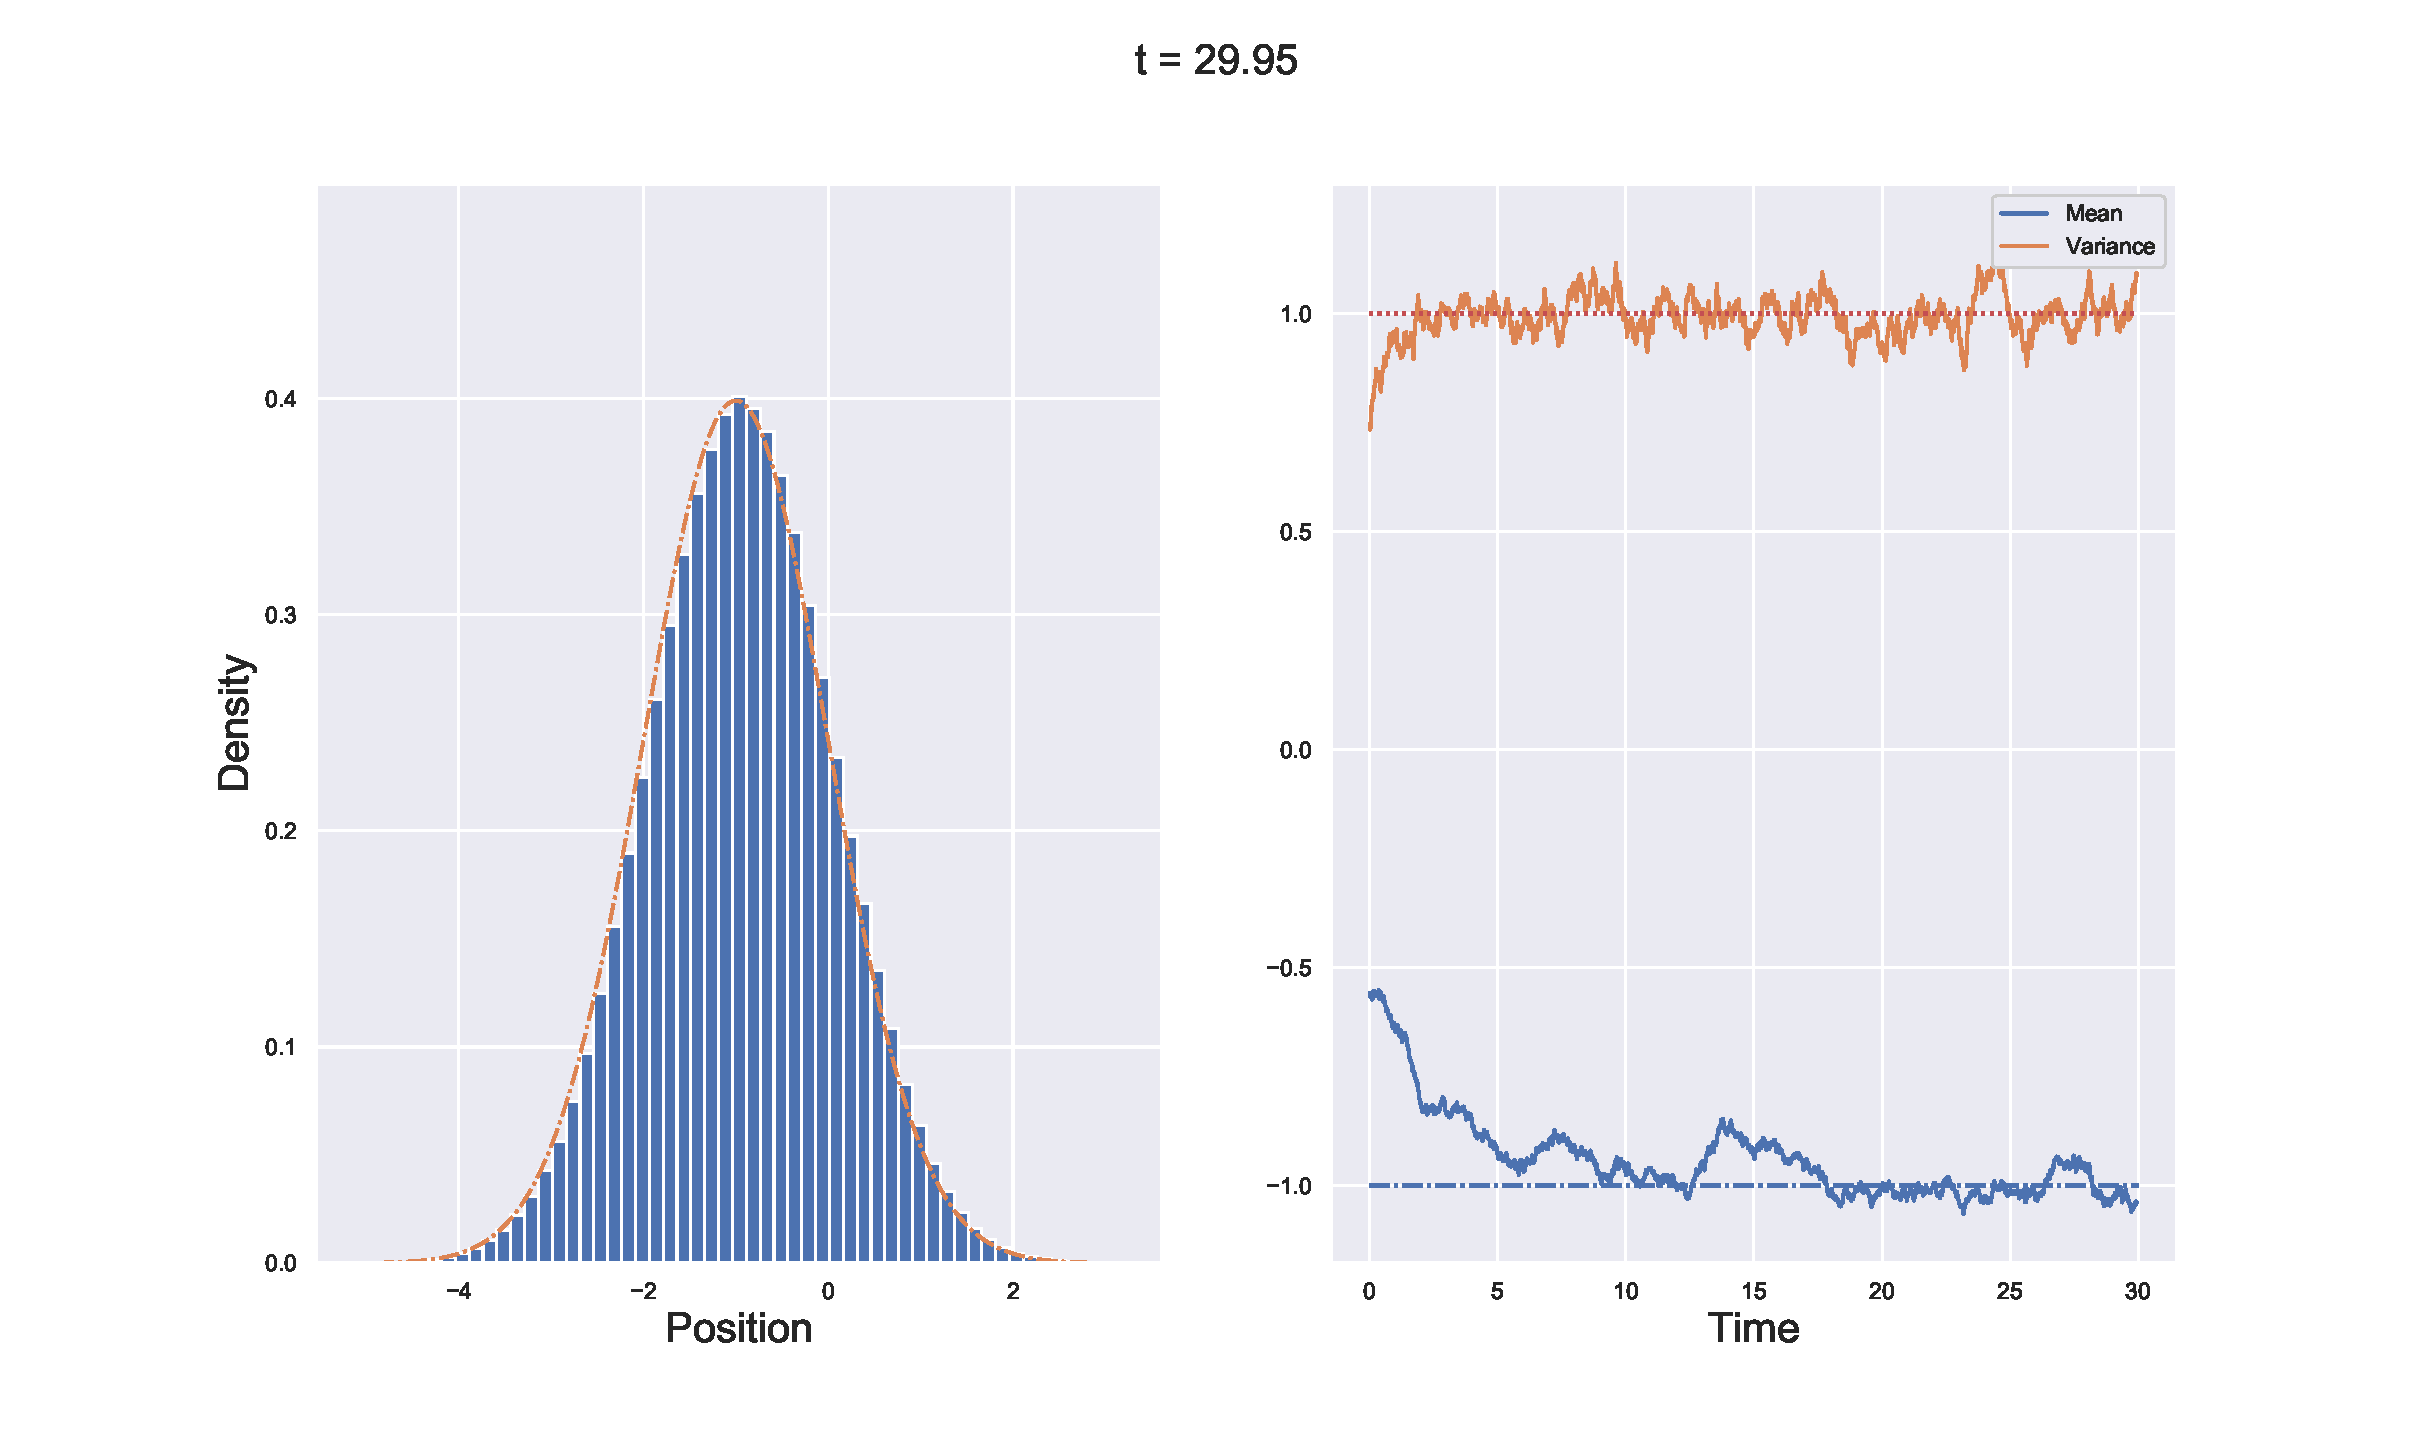
\includegraphics[width=\linewidth]{Figures/homparticles}
    \caption[Homogeneous Particle System]{Histogram of velocities of 1000 particles after 30s with $\sigma = 1$ against the analytic stationary distribution. A time step of $\Dt = 0.01$ was used and the initial data was uniform on $[-2,1]$. The right-hand plot shows the mean and variance moving towards the predicted values and oscillating about them.}
    \label{fig:homparticlemoments}
\end{figure}
We can also plot an animation of the movement of the density of particles over time. Recall from Section \ref{sec:dynamics} that the empirical distribution of the particle system only approximates the true distribution as the number of particles tends to infinity. For any finite number of particles there is only one stationary distribution. When simulating the system, if the number of particles is high enough the probability that enough particles jump across the barrier is very small, and will only be seen if the simulation is ran for an extremely long time. Nevertheless, if the number of particles is low enough, these switches happen often enough to observe, as Figure \ref{fig:switch} shows. This something to be aware of when comparing the kinetic model with the particle model -- a low number of particles produces a better approximation to the invariant distribution of the particle system, but a worse approximation of the kinetic model solution.

\begin{figure}
    \centering
    \includegraphics[width=\linewidth]{Figures/switch}
    \caption[Mean Zero Invariant Measure for the Particle System]{When simulated for a long time with a low number of particles (here there are 6, and $T=500$) the particles do not behave as the kinetic model predicts.}
    \label{fig:switch}
\end{figure}

+++List of things that can be done in code?+++

\subsection{Space-Homogeneous Kinetic Model}\label{sec:homkin}
 Consider the space-homogeneous evolution given by \eqref{eq:spacehomPDE}, that is
    \begin{equation}
    \partial_t f_t(v) = \partial_v vf_t(v) - \partial_v G(\langle w \rangle_{f_t})f_t(v) + \sigma \partial_{vv} f_t(v).\tag{\ref{eq:spacehomPDE}}
    \end{equation}
    Using the methods developed in Section \ref{sec:numericalmethods}, we are now able to approximate this system numerically. As when solving the heat equation, a zero boundary condition shall be enforced. This is valid as we know that the stationary distributions are Gaussian and centred at $-1,0,+1$. The boundary $L$ can then be chosen depending on the the diffusion so that almost no mass is contained beyond the boundary. For example if $\sigma = 1$, the mass contained beyond $L=5$ is of the order $10^{-5}$. 
    
    Simpson's rule will be used as a quick way to approximate the integral within the herding coefficient. To differentiate between the integral and its approximation, we write \(\langle w\rangle_{F^n}\). Below is the scheme when both the herding coefficient and the velocity are positive, using a finite difference scheme with a CN discretisation for the diffusive term and an upwind method for the damping and herding terms.
    \begin{equation*}
    \begin{split}
    \frac{F_j^{n+1} - F_j^n}{\Delta t} = 	-G(\langle w\rangle_{F^n})\left[ \frac{F^n_{j+1} - F^n_{j}}{\Delta v}\right] &+\left[ \frac{v_{j}F^n_{j} - v_{j-1}F^n_{j-1}}{\Delta v}\right]\\ &+ \frac{\sigma}{2}\left[ \frac{F^{n+1}_{j+1} - 2F^{n+1}_j + F^{n+1}_{j-1}}{(\Delta v)^2} + \frac{F^{n}_{j+1} - 2F^{n}_j + F^{n}_{j-1}}{(\Delta v)^2}\right] 	 
    \end{split}
    \end{equation*}
    This scheme will be first order in both time and space due to the use of the first-order upwinding. The stability will be restricted by the CFL condition, in particular, $\frac{|v_j-G(\langle w\rangle_{F^n})|\Dt}{\Dx} \leq 1$. A finite volume scheme has also been implemented. In this scheme the flux out of the right boundary is given by 
     \[ \max(0, v_{j+\frac{1}{2}}-G(\langle w\rangle_{F^n}))F^n_{j+1} + \min(0, v_{j+\frac{1}{2}}-G(\langle w\rangle_{F^n}))F^n_j + \frac{\sigma(F^n_{j+1} - F^n_j)}{\Dv}.
     \]
     This is a simple FTCS method applied to the diffusion term and a first order upwind on the advective term. The stability here is limited by the mesh spacing, however it illustrates the use of a finite volume method without incorporating an implicit solver. Figure +++ref+++ is a frame from an animation of the PDE solution approximated using the finite difference scheme compared with the particle system. The finite difference method appears to closely follow the behaviour of the particle system, so long as the number of particles is high enough. Figure \ref{fig:kinmodelmomvar} shows the first moment and the variance contrasted with the analytic solution of \eqref{eq:momode}. This clearly shows the almost immediate artificial dissipative effects of the upwind scheme in the finite volume case. The finite difference scheme appears to be better approximating the variance, however the spatial bias within this algorithm is not correct. Both schemes report no mass loss to 6 decimal places. This will be the case as long as the initial distribution does not have non-negligible mass at the boundary.
     
     The error in the approximate stationary distribution can be approximated by simply finding the difference between the analytic invariant measure and the approximate solution. Figure \ref{fig:homkinerror} shows exactly this for $\sigma = 1, \Dt = 0.001, T = 20, L=6, \Dv = 0.1$ and Gaussian initial data. The spatial bias in the finite difference method has introduced a bias in the error. No such bias exists for the upwinding in the finite volume solution, although the error is greater. This is very important for our aim in this project. If the initial data has mean zero, the scheme may always converge in the direction of the spatial bias, obscuring the true behaviour. 
    
    \begin{figure}
        \centering
        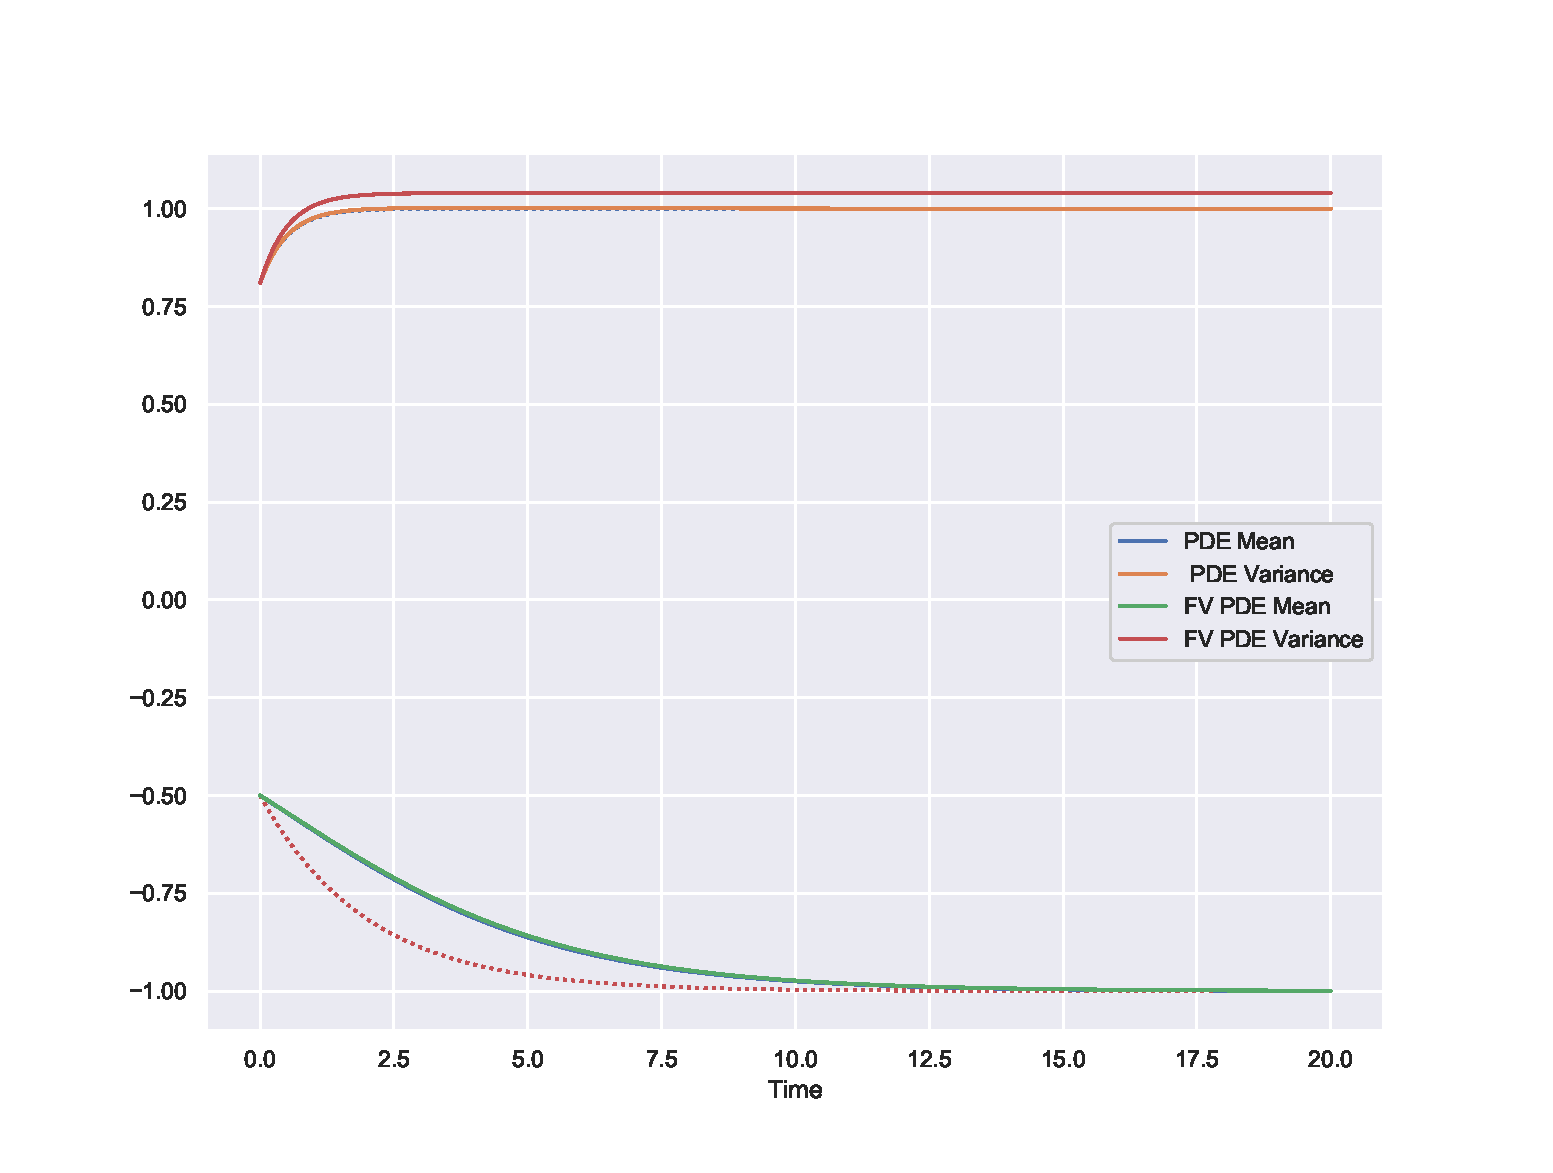
\includegraphics[width=0.7\linewidth]{Figures/kinmodelmomvar}
        \caption[Convergence of Moments for Kinetic Model]{For Gaussian initial data with mean -0.5 and variance 0.81, the schemes both converge with a time step of $\Dt =0.001$ and $\Dv = 0.05$. For the mean, the solvers are almost indistinguishable. The time step must be small so the FTCS scheme within the finite volume solver is stable. Also note the overestimation of variance. }
        \label{fig:kinmodelmomvar}
    \end{figure}

    \begin{figure}
        \centering
        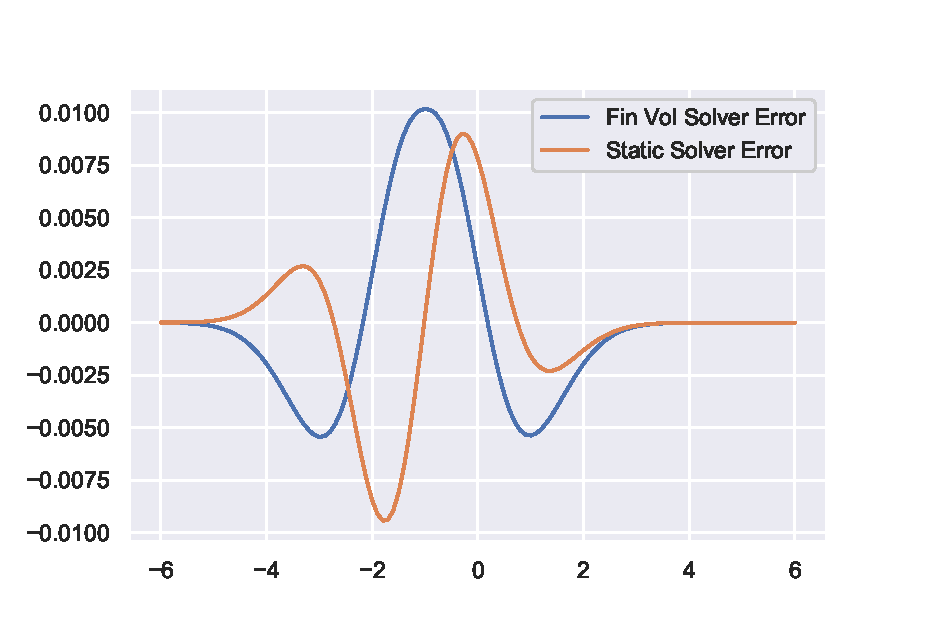
\includegraphics[width=0.7\linewidth]{Figures/homkinerror}
        \caption[Error of the Schemes]{Difference between approximate solution at $t=20$ and a Gaussian distribution with mean -1 and variance 1. Note the spatial bias in the finite difference method has introduced a bias in the error. No such bias exists for the upwinding in the finite volume case.}
        \label{fig:homkinerror}
    \end{figure}
\subsection{Space-Heterogeneous Particle Model}\label{sec:hetkin}
    The next step is to reintroduce the spatial heterogeneity in the particle system. Recall the full particle model is given by
            \begin{equation}\begin{cases}
    \dif x^{i,N}_t = v^{i,N}_t\dif t\\
    \dif v^{i,N}_t = -v^{i,N}_t\dif t + G\left(\frac{\frac{1}{N}\sum_{j=1}^N \phi(x_t^{i,N} - x_t^{j,N})v^{j,N}_t  }{\frac{1}{N}\sum_{j=1}^N \phi(x_t^{i,N} - x_t^{j,N})}\right)\dif t + \sqrt{2\sigma} \dif W^i_t 
    \end{cases}, \qquad  i = 1,\dots,N.\tag{\ref{eq:fullparticle}}
    \end{equation} 
    Letting $\phi\equiv 1$ forces the interaction to be homogeneous in space still, however there is now the movement of particles in space given by the first equation. 
    